% Created by tikzDevice version 0.6.2-92-0ad2792 on 2013-11-12 07:32:23
% !TEX encoding = UTF-8 Unicode
\documentclass[12pt, mainfont = Minion,     mainscale = 1.0, sansfont = Myriad,     sansscale = MatchLowercase, monofont = Consolas,   monoscale = MatchLowercase, mathfont = MinionMath, mathscale = 1.0]{mtikzfig}
\begin{document}

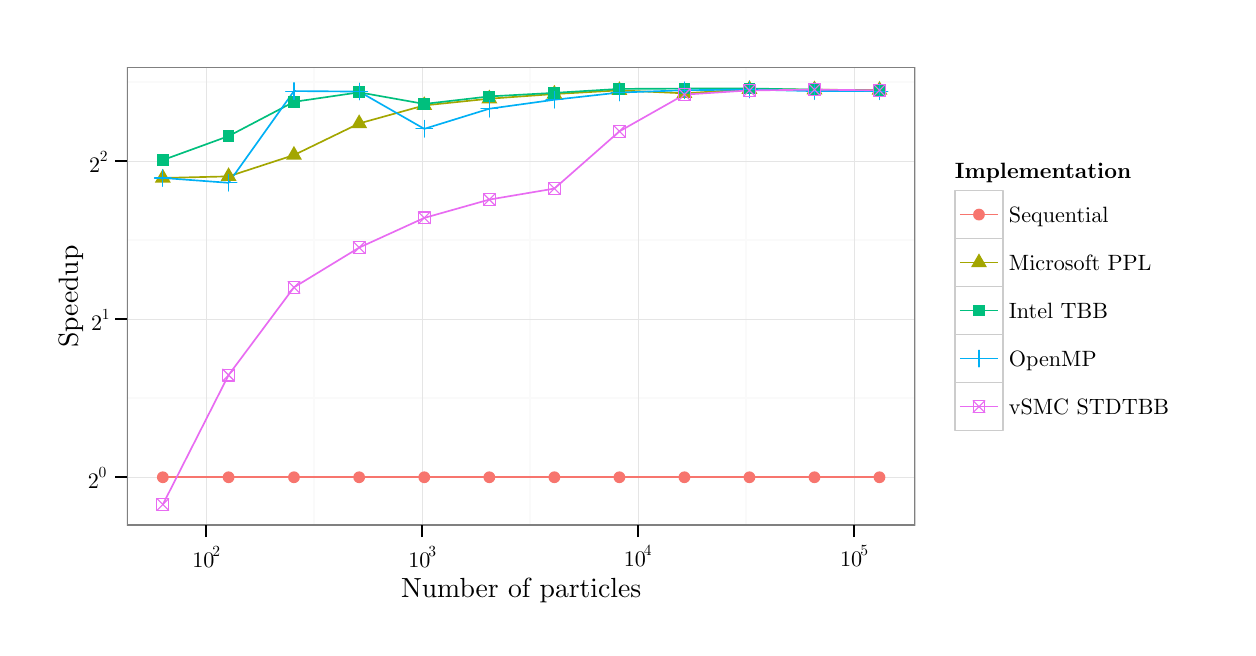
\begin{tikzpicture}[x=1pt,y=1pt]
\definecolor[named]{fillColor}{rgb}{1.00,1.00,1.00}
\path[use as bounding box,fill=fillColor,fill opacity=0.00] (0,0) rectangle (433.62,216.81);
\begin{scope}
\path[clip] (  0.00,  0.00) rectangle (433.62,216.81);
\definecolor[named]{drawColor}{rgb}{1.00,1.00,1.00}
\definecolor[named]{fillColor}{rgb}{1.00,1.00,1.00}

\path[draw=drawColor,line width= 0.6pt,line join=round,line cap=round,fill=fillColor] ( -0.00,  0.00) rectangle (433.62,216.81);
\end{scope}
\begin{scope}
\path[clip] ( 35.89, 37.00) rectangle (320.74,202.36);
\definecolor[named]{fillColor}{rgb}{1.00,1.00,1.00}

\path[fill=fillColor] ( 35.89, 37.00) rectangle (320.74,202.36);
\definecolor[named]{drawColor}{rgb}{0.98,0.98,0.98}

\path[draw=drawColor,line width= 0.6pt,line join=round] ( 35.89, 82.90) --
	(320.74, 82.90);

\path[draw=drawColor,line width= 0.6pt,line join=round] ( 35.89,140.00) --
	(320.74,140.00);

\path[draw=drawColor,line width= 0.6pt,line join=round] ( 35.89,197.09) --
	(320.74,197.09);

\path[draw=drawColor,line width= 0.6pt,line join=round] (103.52, 37.00) --
	(103.52,202.36);

\path[draw=drawColor,line width= 0.6pt,line join=round] (181.56, 37.00) --
	(181.56,202.36);

\path[draw=drawColor,line width= 0.6pt,line join=round] (259.60, 37.00) --
	(259.60,202.36);
\definecolor[named]{drawColor}{rgb}{0.90,0.90,0.90}

\path[draw=drawColor,line width= 0.2pt,line join=round] ( 35.89, 54.35) --
	(320.74, 54.35);

\path[draw=drawColor,line width= 0.2pt,line join=round] ( 35.89,111.45) --
	(320.74,111.45);

\path[draw=drawColor,line width= 0.2pt,line join=round] ( 35.89,168.55) --
	(320.74,168.55);

\path[draw=drawColor,line width= 0.2pt,line join=round] ( 64.50, 37.00) --
	( 64.50,202.36);

\path[draw=drawColor,line width= 0.2pt,line join=round] (142.54, 37.00) --
	(142.54,202.36);

\path[draw=drawColor,line width= 0.2pt,line join=round] (220.58, 37.00) --
	(220.58,202.36);

\path[draw=drawColor,line width= 0.2pt,line join=round] (298.62, 37.00) --
	(298.62,202.36);
\definecolor[named]{drawColor}{rgb}{0.97,0.46,0.43}

\path[draw=drawColor,line width= 0.6pt,line join=round] ( 48.84, 54.35) --
	( 72.60, 54.35) --
	( 96.22, 54.35) --
	(119.78, 54.35) --
	(143.31, 54.35) --
	(166.82, 54.35) --
	(190.32, 54.35) --
	(213.82, 54.35) --
	(237.31, 54.35) --
	(260.81, 54.35) --
	(284.30, 54.35) --
	(307.79, 54.35);
\definecolor[named]{drawColor}{rgb}{0.64,0.65,0.00}

\path[draw=drawColor,line width= 0.6pt,line join=round] ( 48.84,162.50) --
	( 72.60,163.07) --
	( 96.22,170.77) --
	(119.78,182.20) --
	(143.31,188.72) --
	(166.82,191.14) --
	(190.32,192.83) --
	(213.82,194.15) --
	(237.31,193.08) --
	(260.81,194.55) --
	(284.30,194.40) --
	(307.79,194.25);
\definecolor[named]{drawColor}{rgb}{0.00,0.75,0.49}

\path[draw=drawColor,line width= 0.6pt,line join=round] ( 48.84,168.97) --
	( 72.60,177.62) --
	( 96.22,190.01) --
	(119.78,193.44) --
	(143.31,189.25) --
	(166.82,191.97) --
	(190.32,193.25) --
	(213.82,194.68) --
	(237.31,194.80) --
	(260.81,194.84) --
	(284.30,194.40) --
	(307.79,193.99);
\definecolor[named]{drawColor}{rgb}{0.00,0.69,0.96}

\path[draw=drawColor,line width= 0.6pt,line join=round] ( 48.84,162.50) --
	( 72.60,160.75) --
	( 96.22,193.90) --
	(119.78,193.72) --
	(143.31,180.25) --
	(166.82,187.52) --
	(190.32,190.76) --
	(213.82,193.37) --
	(237.31,194.20) --
	(260.81,194.45) --
	(284.30,193.89) --
	(307.79,193.86);
\definecolor[named]{drawColor}{rgb}{0.91,0.42,0.95}

\path[draw=drawColor,line width= 0.6pt,line join=round] ( 48.84, 44.51) --
	( 72.60, 91.29) --
	( 96.22,122.97) --
	(119.78,137.33) --
	(143.31,148.06) --
	(166.82,154.69) --
	(190.32,158.66) --
	(213.82,179.34) --
	(237.31,192.62) --
	(260.81,194.14) --
	(284.30,194.40) --
	(307.79,194.17);
\definecolor[named]{fillColor}{rgb}{0.97,0.46,0.43}

\path[fill=fillColor] ( 48.84, 54.35) circle (  2.13);
\definecolor[named]{fillColor}{rgb}{0.64,0.65,0.00}

\path[fill=fillColor] ( 48.84,165.82) --
	( 51.71,160.84) --
	( 45.96,160.84) --
	cycle;
\definecolor[named]{fillColor}{rgb}{0.00,0.75,0.49}

\path[fill=fillColor] ( 46.70,166.83) --
	( 50.97,166.83) --
	( 50.97,171.10) --
	( 46.70,171.10) --
	cycle;
\definecolor[named]{drawColor}{rgb}{0.00,0.69,0.96}

\path[draw=drawColor,line width= 0.4pt,line join=round,line cap=round] ( 45.82,162.50) -- ( 51.86,162.50);

\path[draw=drawColor,line width= 0.4pt,line join=round,line cap=round] ( 48.84,159.48) -- ( 48.84,165.52);
\definecolor[named]{drawColor}{rgb}{0.91,0.42,0.95}

\path[draw=drawColor,line width= 0.4pt,line join=round,line cap=round] ( 46.70, 42.38) rectangle ( 50.97, 46.65);

\path[draw=drawColor,line width= 0.4pt,line join=round,line cap=round] ( 46.70, 42.38) -- ( 50.97, 46.65);

\path[draw=drawColor,line width= 0.4pt,line join=round,line cap=round] ( 46.70, 46.65) -- ( 50.97, 42.38);
\definecolor[named]{fillColor}{rgb}{0.97,0.46,0.43}

\path[fill=fillColor] ( 72.60, 54.35) circle (  2.13);
\definecolor[named]{fillColor}{rgb}{0.64,0.65,0.00}

\path[fill=fillColor] ( 72.60,166.39) --
	( 75.47,161.41) --
	( 69.72,161.41) --
	cycle;
\definecolor[named]{fillColor}{rgb}{0.00,0.75,0.49}

\path[fill=fillColor] ( 70.46,175.49) --
	( 74.73,175.49) --
	( 74.73,179.76) --
	( 70.46,179.76) --
	cycle;
\definecolor[named]{drawColor}{rgb}{0.00,0.69,0.96}

\path[draw=drawColor,line width= 0.4pt,line join=round,line cap=round] ( 69.58,160.75) -- ( 75.62,160.75);

\path[draw=drawColor,line width= 0.4pt,line join=round,line cap=round] ( 72.60,157.74) -- ( 72.60,163.77);
\definecolor[named]{drawColor}{rgb}{0.91,0.42,0.95}

\path[draw=drawColor,line width= 0.4pt,line join=round,line cap=round] ( 70.46, 89.15) rectangle ( 74.73, 93.42);

\path[draw=drawColor,line width= 0.4pt,line join=round,line cap=round] ( 70.46, 89.15) -- ( 74.73, 93.42);

\path[draw=drawColor,line width= 0.4pt,line join=round,line cap=round] ( 70.46, 93.42) -- ( 74.73, 89.15);
\definecolor[named]{fillColor}{rgb}{0.97,0.46,0.43}

\path[fill=fillColor] ( 96.22, 54.35) circle (  2.13);
\definecolor[named]{fillColor}{rgb}{0.64,0.65,0.00}

\path[fill=fillColor] ( 96.22,174.09) --
	( 99.10,169.11) --
	( 93.35,169.11) --
	cycle;
\definecolor[named]{fillColor}{rgb}{0.00,0.75,0.49}

\path[fill=fillColor] ( 94.09,187.88) --
	( 98.36,187.88) --
	( 98.36,192.15) --
	( 94.09,192.15) --
	cycle;
\definecolor[named]{drawColor}{rgb}{0.00,0.69,0.96}

\path[draw=drawColor,line width= 0.4pt,line join=round,line cap=round] ( 93.21,193.90) -- ( 99.24,193.90);

\path[draw=drawColor,line width= 0.4pt,line join=round,line cap=round] ( 96.22,190.88) -- ( 96.22,196.91);
\definecolor[named]{drawColor}{rgb}{0.91,0.42,0.95}

\path[draw=drawColor,line width= 0.4pt,line join=round,line cap=round] ( 94.09,120.84) rectangle ( 98.36,125.11);

\path[draw=drawColor,line width= 0.4pt,line join=round,line cap=round] ( 94.09,120.84) -- ( 98.36,125.11);

\path[draw=drawColor,line width= 0.4pt,line join=round,line cap=round] ( 94.09,125.11) -- ( 98.36,120.84);
\definecolor[named]{fillColor}{rgb}{0.97,0.46,0.43}

\path[fill=fillColor] (119.78, 54.35) circle (  2.13);
\definecolor[named]{fillColor}{rgb}{0.64,0.65,0.00}

\path[fill=fillColor] (119.78,185.52) --
	(122.66,180.54) --
	(116.91,180.54) --
	cycle;
\definecolor[named]{fillColor}{rgb}{0.00,0.75,0.49}

\path[fill=fillColor] (117.65,191.31) --
	(121.92,191.31) --
	(121.92,195.58) --
	(117.65,195.58) --
	cycle;
\definecolor[named]{drawColor}{rgb}{0.00,0.69,0.96}

\path[draw=drawColor,line width= 0.4pt,line join=round,line cap=round] (116.77,193.72) -- (122.80,193.72);

\path[draw=drawColor,line width= 0.4pt,line join=round,line cap=round] (119.78,190.71) -- (119.78,196.74);
\definecolor[named]{drawColor}{rgb}{0.91,0.42,0.95}

\path[draw=drawColor,line width= 0.4pt,line join=round,line cap=round] (117.65,135.20) rectangle (121.92,139.47);

\path[draw=drawColor,line width= 0.4pt,line join=round,line cap=round] (117.65,135.20) -- (121.92,139.47);

\path[draw=drawColor,line width= 0.4pt,line join=round,line cap=round] (117.65,139.47) -- (121.92,135.20);
\definecolor[named]{fillColor}{rgb}{0.97,0.46,0.43}

\path[fill=fillColor] (143.31, 54.35) circle (  2.13);
\definecolor[named]{fillColor}{rgb}{0.64,0.65,0.00}

\path[fill=fillColor] (143.31,192.04) --
	(146.18,187.06) --
	(140.44,187.06) --
	cycle;
\definecolor[named]{fillColor}{rgb}{0.00,0.75,0.49}

\path[fill=fillColor] (141.18,187.12) --
	(145.44,187.12) --
	(145.44,191.39) --
	(141.18,191.39) --
	cycle;
\definecolor[named]{drawColor}{rgb}{0.00,0.69,0.96}

\path[draw=drawColor,line width= 0.4pt,line join=round,line cap=round] (140.29,180.25) -- (146.33,180.25);

\path[draw=drawColor,line width= 0.4pt,line join=round,line cap=round] (143.31,177.23) -- (143.31,183.27);
\definecolor[named]{drawColor}{rgb}{0.91,0.42,0.95}

\path[draw=drawColor,line width= 0.4pt,line join=round,line cap=round] (141.18,145.93) rectangle (145.44,150.20);

\path[draw=drawColor,line width= 0.4pt,line join=round,line cap=round] (141.18,145.93) -- (145.44,150.20);

\path[draw=drawColor,line width= 0.4pt,line join=round,line cap=round] (141.18,150.20) -- (145.44,145.93);
\definecolor[named]{fillColor}{rgb}{0.97,0.46,0.43}

\path[fill=fillColor] (166.82, 54.35) circle (  2.13);
\definecolor[named]{fillColor}{rgb}{0.64,0.65,0.00}

\path[fill=fillColor] (166.82,194.46) --
	(169.69,189.48) --
	(163.95,189.48) --
	cycle;
\definecolor[named]{fillColor}{rgb}{0.00,0.75,0.49}

\path[fill=fillColor] (164.69,189.84) --
	(168.95,189.84) --
	(168.95,194.10) --
	(164.69,194.10) --
	cycle;
\definecolor[named]{drawColor}{rgb}{0.00,0.69,0.96}

\path[draw=drawColor,line width= 0.4pt,line join=round,line cap=round] (163.80,187.52) -- (169.84,187.52);

\path[draw=drawColor,line width= 0.4pt,line join=round,line cap=round] (166.82,184.50) -- (166.82,190.53);
\definecolor[named]{drawColor}{rgb}{0.91,0.42,0.95}

\path[draw=drawColor,line width= 0.4pt,line join=round,line cap=round] (164.69,152.55) rectangle (168.95,156.82);

\path[draw=drawColor,line width= 0.4pt,line join=round,line cap=round] (164.69,152.55) -- (168.95,156.82);

\path[draw=drawColor,line width= 0.4pt,line join=round,line cap=round] (164.69,156.82) -- (168.95,152.55);
\definecolor[named]{fillColor}{rgb}{0.97,0.46,0.43}

\path[fill=fillColor] (190.32, 54.35) circle (  2.13);
\definecolor[named]{fillColor}{rgb}{0.64,0.65,0.00}

\path[fill=fillColor] (190.32,196.15) --
	(193.19,191.17) --
	(187.45,191.17) --
	cycle;
\definecolor[named]{fillColor}{rgb}{0.00,0.75,0.49}

\path[fill=fillColor] (188.19,191.12) --
	(192.45,191.12) --
	(192.45,195.38) --
	(188.19,195.38) --
	cycle;
\definecolor[named]{drawColor}{rgb}{0.00,0.69,0.96}

\path[draw=drawColor,line width= 0.4pt,line join=round,line cap=round] (187.30,190.76) -- (193.34,190.76);

\path[draw=drawColor,line width= 0.4pt,line join=round,line cap=round] (190.32,187.74) -- (190.32,193.78);
\definecolor[named]{drawColor}{rgb}{0.91,0.42,0.95}

\path[draw=drawColor,line width= 0.4pt,line join=round,line cap=round] (188.19,156.53) rectangle (192.45,160.80);

\path[draw=drawColor,line width= 0.4pt,line join=round,line cap=round] (188.19,156.53) -- (192.45,160.80);

\path[draw=drawColor,line width= 0.4pt,line join=round,line cap=round] (188.19,160.80) -- (192.45,156.53);
\definecolor[named]{fillColor}{rgb}{0.97,0.46,0.43}

\path[fill=fillColor] (213.82, 54.35) circle (  2.13);
\definecolor[named]{fillColor}{rgb}{0.64,0.65,0.00}

\path[fill=fillColor] (213.82,197.47) --
	(216.69,192.49) --
	(210.94,192.49) --
	cycle;
\definecolor[named]{fillColor}{rgb}{0.00,0.75,0.49}

\path[fill=fillColor] (211.68,192.55) --
	(215.95,192.55) --
	(215.95,196.81) --
	(211.68,196.81) --
	cycle;
\definecolor[named]{drawColor}{rgb}{0.00,0.69,0.96}

\path[draw=drawColor,line width= 0.4pt,line join=round,line cap=round] (210.80,193.37) -- (216.84,193.37);

\path[draw=drawColor,line width= 0.4pt,line join=round,line cap=round] (213.82,190.35) -- (213.82,196.39);
\definecolor[named]{drawColor}{rgb}{0.91,0.42,0.95}

\path[draw=drawColor,line width= 0.4pt,line join=round,line cap=round] (211.68,177.21) rectangle (215.95,181.48);

\path[draw=drawColor,line width= 0.4pt,line join=round,line cap=round] (211.68,177.21) -- (215.95,181.48);

\path[draw=drawColor,line width= 0.4pt,line join=round,line cap=round] (211.68,181.48) -- (215.95,177.21);
\definecolor[named]{fillColor}{rgb}{0.97,0.46,0.43}

\path[fill=fillColor] (237.31, 54.35) circle (  2.13);
\definecolor[named]{fillColor}{rgb}{0.64,0.65,0.00}

\path[fill=fillColor] (237.31,196.40) --
	(240.19,191.42) --
	(234.44,191.42) --
	cycle;
\definecolor[named]{fillColor}{rgb}{0.00,0.75,0.49}

\path[fill=fillColor] (235.18,192.66) --
	(239.45,192.66) --
	(239.45,196.93) --
	(235.18,196.93) --
	cycle;
\definecolor[named]{drawColor}{rgb}{0.00,0.69,0.96}

\path[draw=drawColor,line width= 0.4pt,line join=round,line cap=round] (234.29,194.20) -- (240.33,194.20);

\path[draw=drawColor,line width= 0.4pt,line join=round,line cap=round] (237.31,191.18) -- (237.31,197.22);
\definecolor[named]{drawColor}{rgb}{0.91,0.42,0.95}

\path[draw=drawColor,line width= 0.4pt,line join=round,line cap=round] (235.18,190.49) rectangle (239.45,194.76);

\path[draw=drawColor,line width= 0.4pt,line join=round,line cap=round] (235.18,190.49) -- (239.45,194.76);

\path[draw=drawColor,line width= 0.4pt,line join=round,line cap=round] (235.18,194.76) -- (239.45,190.49);
\definecolor[named]{fillColor}{rgb}{0.97,0.46,0.43}

\path[fill=fillColor] (260.81, 54.35) circle (  2.13);
\definecolor[named]{fillColor}{rgb}{0.64,0.65,0.00}

\path[fill=fillColor] (260.81,197.87) --
	(263.68,192.89) --
	(257.93,192.89) --
	cycle;
\definecolor[named]{fillColor}{rgb}{0.00,0.75,0.49}

\path[fill=fillColor] (258.67,192.71) --
	(262.94,192.71) --
	(262.94,196.97) --
	(258.67,196.97) --
	cycle;
\definecolor[named]{drawColor}{rgb}{0.00,0.69,0.96}

\path[draw=drawColor,line width= 0.4pt,line join=round,line cap=round] (257.79,194.45) -- (263.82,194.45);

\path[draw=drawColor,line width= 0.4pt,line join=round,line cap=round] (260.81,191.43) -- (260.81,197.47);
\definecolor[named]{drawColor}{rgb}{0.91,0.42,0.95}

\path[draw=drawColor,line width= 0.4pt,line join=round,line cap=round] (258.67,192.00) rectangle (262.94,196.27);

\path[draw=drawColor,line width= 0.4pt,line join=round,line cap=round] (258.67,192.00) -- (262.94,196.27);

\path[draw=drawColor,line width= 0.4pt,line join=round,line cap=round] (258.67,196.27) -- (262.94,192.00);
\definecolor[named]{fillColor}{rgb}{0.97,0.46,0.43}

\path[fill=fillColor] (284.30, 54.35) circle (  2.13);
\definecolor[named]{fillColor}{rgb}{0.64,0.65,0.00}

\path[fill=fillColor] (284.30,197.72) --
	(287.17,192.74) --
	(281.43,192.74) --
	cycle;
\definecolor[named]{fillColor}{rgb}{0.00,0.75,0.49}

\path[fill=fillColor] (282.17,192.26) --
	(286.43,192.26) --
	(286.43,196.53) --
	(282.17,196.53) --
	cycle;
\definecolor[named]{drawColor}{rgb}{0.00,0.69,0.96}

\path[draw=drawColor,line width= 0.4pt,line join=round,line cap=round] (281.28,193.89) -- (287.32,193.89);

\path[draw=drawColor,line width= 0.4pt,line join=round,line cap=round] (284.30,190.87) -- (284.30,196.90);
\definecolor[named]{drawColor}{rgb}{0.91,0.42,0.95}

\path[draw=drawColor,line width= 0.4pt,line join=round,line cap=round] (282.17,192.27) rectangle (286.43,196.54);

\path[draw=drawColor,line width= 0.4pt,line join=round,line cap=round] (282.17,192.27) -- (286.43,196.54);

\path[draw=drawColor,line width= 0.4pt,line join=round,line cap=round] (282.17,196.54) -- (286.43,192.27);
\definecolor[named]{fillColor}{rgb}{0.97,0.46,0.43}

\path[fill=fillColor] (307.79, 54.35) circle (  2.13);
\definecolor[named]{fillColor}{rgb}{0.64,0.65,0.00}

\path[fill=fillColor] (307.79,197.57) --
	(310.67,192.59) --
	(304.92,192.59) --
	cycle;
\definecolor[named]{fillColor}{rgb}{0.00,0.75,0.49}

\path[fill=fillColor] (305.66,191.86) --
	(309.93,191.86) --
	(309.93,196.13) --
	(305.66,196.13) --
	cycle;
\definecolor[named]{drawColor}{rgb}{0.00,0.69,0.96}

\path[draw=drawColor,line width= 0.4pt,line join=round,line cap=round] (304.78,193.86) -- (310.81,193.86);

\path[draw=drawColor,line width= 0.4pt,line join=round,line cap=round] (307.79,190.84) -- (307.79,196.87);
\definecolor[named]{drawColor}{rgb}{0.91,0.42,0.95}

\path[draw=drawColor,line width= 0.4pt,line join=round,line cap=round] (305.66,192.04) rectangle (309.93,196.30);

\path[draw=drawColor,line width= 0.4pt,line join=round,line cap=round] (305.66,192.04) -- (309.93,196.30);

\path[draw=drawColor,line width= 0.4pt,line join=round,line cap=round] (305.66,196.30) -- (309.93,192.04);
\definecolor[named]{drawColor}{rgb}{0.50,0.50,0.50}

\path[draw=drawColor,line width= 0.6pt,line join=round,line cap=round] ( 35.89, 37.00) rectangle (320.74,202.36);
\end{scope}
\begin{scope}
\path[clip] (  0.00,  0.00) rectangle (433.62,216.81);
\definecolor[named]{drawColor}{rgb}{0.00,0.00,0.00}

\node[text=drawColor,anchor=base west,inner sep=0pt, outer sep=0pt, scale=  0.80] at ( 21.77, 50.35) {2};

\node[text=drawColor,anchor=base west,inner sep=0pt, outer sep=0pt, scale=  0.56] at ( 25.66, 54.34) {0};

\node[text=drawColor,anchor=base west,inner sep=0pt, outer sep=0pt, scale=  0.80] at ( 22.91,107.48) {2};

\node[text=drawColor,anchor=base west,inner sep=0pt, outer sep=0pt, scale=  0.56] at ( 26.79,111.47) {1};

\node[text=drawColor,anchor=base west,inner sep=0pt, outer sep=0pt, scale=  0.80] at ( 22.17,164.54) {2};

\node[text=drawColor,anchor=base west,inner sep=0pt, outer sep=0pt, scale=  0.56] at ( 26.06,168.53) {2};
\end{scope}
\begin{scope}
\path[clip] (  0.00,  0.00) rectangle (433.62,216.81);
\definecolor[named]{drawColor}{rgb}{0.00,0.00,0.00}

\path[draw=drawColor,line width= 0.6pt,line join=round] ( 31.62, 54.35) --
	( 35.89, 54.35);

\path[draw=drawColor,line width= 0.6pt,line join=round] ( 31.62,111.45) --
	( 35.89,111.45);

\path[draw=drawColor,line width= 0.6pt,line join=round] ( 31.62,168.55) --
	( 35.89,168.55);
\end{scope}
\begin{scope}
\path[clip] (  0.00,  0.00) rectangle (433.62,216.81);
\definecolor[named]{drawColor}{rgb}{0.00,0.00,0.00}

\path[draw=drawColor,line width= 0.6pt,line join=round] ( 64.50, 32.73) --
	( 64.50, 37.00);

\path[draw=drawColor,line width= 0.6pt,line join=round] (142.54, 32.73) --
	(142.54, 37.00);

\path[draw=drawColor,line width= 0.6pt,line join=round] (220.58, 32.73) --
	(220.58, 37.00);

\path[draw=drawColor,line width= 0.6pt,line join=round] (298.62, 32.73) --
	(298.62, 37.00);
\end{scope}
\begin{scope}
\path[clip] (  0.00,  0.00) rectangle (433.62,216.81);
\definecolor[named]{drawColor}{rgb}{0.00,0.00,0.00}

\node[text=drawColor,anchor=base west,inner sep=0pt, outer sep=0pt, scale=  0.80] at ( 59.49, 21.87) {10};

\node[text=drawColor,anchor=base west,inner sep=0pt, outer sep=0pt, scale=  0.56] at ( 66.78, 25.86) {2};

\node[text=drawColor,anchor=base west,inner sep=0pt, outer sep=0pt, scale=  0.80] at (137.53, 21.87) {10};

\node[text=drawColor,anchor=base west,inner sep=0pt, outer sep=0pt, scale=  0.56] at (144.82, 25.86) {3};

\node[text=drawColor,anchor=base west,inner sep=0pt, outer sep=0pt, scale=  0.80] at (215.41, 21.94) {10};

\node[text=drawColor,anchor=base west,inner sep=0pt, outer sep=0pt, scale=  0.56] at (222.70, 25.93) {4};

\node[text=drawColor,anchor=base west,inner sep=0pt, outer sep=0pt, scale=  0.80] at (293.58, 21.94) {10};

\node[text=drawColor,anchor=base west,inner sep=0pt, outer sep=0pt, scale=  0.56] at (300.87, 25.93) {5};
\end{scope}
\begin{scope}
\path[clip] (  0.00,  0.00) rectangle (433.62,216.81);
\definecolor[named]{drawColor}{rgb}{0.00,0.00,0.00}

\node[text=drawColor,anchor=base,inner sep=0pt, outer sep=0pt, scale=  1.00] at (178.32, 10.84) {Number of particles};
\end{scope}
\begin{scope}
\path[clip] (  0.00,  0.00) rectangle (433.62,216.81);
\definecolor[named]{drawColor}{rgb}{0.00,0.00,0.00}

\node[text=drawColor,rotate= 90.00,anchor=base,inner sep=0pt, outer sep=0pt, scale=  1.00] at ( 18.16,119.68) {Speedup};
\end{scope}
\begin{scope}
\path[clip] (  0.00,  0.00) rectangle (433.62,216.81);
\definecolor[named]{fillColor}{rgb}{1.00,1.00,1.00}

\path[fill=fillColor] (330.81, 66.95) rectangle (409.09,172.40);
\end{scope}
\begin{scope}
\path[clip] (  0.00,  0.00) rectangle (433.62,216.81);
\definecolor[named]{drawColor}{rgb}{0.00,0.00,0.00}

\node[text=drawColor,anchor=base west,inner sep=0pt, outer sep=0pt, scale=  0.80] at (335.08,162.28) {\bfseries Implementation};
\end{scope}
\begin{scope}
\path[clip] (  0.00,  0.00) rectangle (433.62,216.81);
\definecolor[named]{drawColor}{rgb}{0.80,0.80,0.80}
\definecolor[named]{fillColor}{rgb}{1.00,1.00,1.00}

\path[draw=drawColor,line width= 0.6pt,line join=round,line cap=round,fill=fillColor] (335.08,140.60) rectangle (352.43,157.94);
\end{scope}
\begin{scope}
\path[clip] (  0.00,  0.00) rectangle (433.62,216.81);
\definecolor[named]{drawColor}{rgb}{0.97,0.46,0.43}

\path[draw=drawColor,line width= 0.6pt,line join=round] (336.82,149.27) -- (350.69,149.27);
\end{scope}
\begin{scope}
\path[clip] (  0.00,  0.00) rectangle (433.62,216.81);
\definecolor[named]{fillColor}{rgb}{0.97,0.46,0.43}

\path[fill=fillColor] (343.75,149.27) circle (  2.13);
\end{scope}
\begin{scope}
\path[clip] (  0.00,  0.00) rectangle (433.62,216.81);
\definecolor[named]{drawColor}{rgb}{0.80,0.80,0.80}
\definecolor[named]{fillColor}{rgb}{1.00,1.00,1.00}

\path[draw=drawColor,line width= 0.6pt,line join=round,line cap=round,fill=fillColor] (335.08,123.25) rectangle (352.43,140.60);
\end{scope}
\begin{scope}
\path[clip] (  0.00,  0.00) rectangle (433.62,216.81);
\definecolor[named]{drawColor}{rgb}{0.64,0.65,0.00}

\path[draw=drawColor,line width= 0.6pt,line join=round] (336.82,131.93) -- (350.69,131.93);
\end{scope}
\begin{scope}
\path[clip] (  0.00,  0.00) rectangle (433.62,216.81);
\definecolor[named]{fillColor}{rgb}{0.64,0.65,0.00}

\path[fill=fillColor] (343.75,135.24) --
	(346.63,130.27) --
	(340.88,130.27) --
	cycle;
\end{scope}
\begin{scope}
\path[clip] (  0.00,  0.00) rectangle (433.62,216.81);
\definecolor[named]{drawColor}{rgb}{0.80,0.80,0.80}
\definecolor[named]{fillColor}{rgb}{1.00,1.00,1.00}

\path[draw=drawColor,line width= 0.6pt,line join=round,line cap=round,fill=fillColor] (335.08,105.91) rectangle (352.43,123.25);
\end{scope}
\begin{scope}
\path[clip] (  0.00,  0.00) rectangle (433.62,216.81);
\definecolor[named]{drawColor}{rgb}{0.00,0.75,0.49}

\path[draw=drawColor,line width= 0.6pt,line join=round] (336.82,114.58) -- (350.69,114.58);
\end{scope}
\begin{scope}
\path[clip] (  0.00,  0.00) rectangle (433.62,216.81);
\definecolor[named]{fillColor}{rgb}{0.00,0.75,0.49}

\path[fill=fillColor] (341.62,112.45) --
	(345.89,112.45) --
	(345.89,116.71) --
	(341.62,116.71) --
	cycle;
\end{scope}
\begin{scope}
\path[clip] (  0.00,  0.00) rectangle (433.62,216.81);
\definecolor[named]{drawColor}{rgb}{0.80,0.80,0.80}
\definecolor[named]{fillColor}{rgb}{1.00,1.00,1.00}

\path[draw=drawColor,line width= 0.6pt,line join=round,line cap=round,fill=fillColor] (335.08, 88.56) rectangle (352.43,105.91);
\end{scope}
\begin{scope}
\path[clip] (  0.00,  0.00) rectangle (433.62,216.81);
\definecolor[named]{drawColor}{rgb}{0.00,0.69,0.96}

\path[draw=drawColor,line width= 0.6pt,line join=round] (336.82, 97.24) -- (350.69, 97.24);
\end{scope}
\begin{scope}
\path[clip] (  0.00,  0.00) rectangle (433.62,216.81);
\definecolor[named]{drawColor}{rgb}{0.00,0.69,0.96}

\path[draw=drawColor,line width= 0.4pt,line join=round,line cap=round] (340.74, 97.24) -- (346.77, 97.24);

\path[draw=drawColor,line width= 0.4pt,line join=round,line cap=round] (343.75, 94.22) -- (343.75,100.25);
\end{scope}
\begin{scope}
\path[clip] (  0.00,  0.00) rectangle (433.62,216.81);
\definecolor[named]{drawColor}{rgb}{0.80,0.80,0.80}
\definecolor[named]{fillColor}{rgb}{1.00,1.00,1.00}

\path[draw=drawColor,line width= 0.6pt,line join=round,line cap=round,fill=fillColor] (335.08, 71.22) rectangle (352.43, 88.56);
\end{scope}
\begin{scope}
\path[clip] (  0.00,  0.00) rectangle (433.62,216.81);
\definecolor[named]{drawColor}{rgb}{0.91,0.42,0.95}

\path[draw=drawColor,line width= 0.6pt,line join=round] (336.82, 79.89) -- (350.69, 79.89);
\end{scope}
\begin{scope}
\path[clip] (  0.00,  0.00) rectangle (433.62,216.81);
\definecolor[named]{drawColor}{rgb}{0.91,0.42,0.95}

\path[draw=drawColor,line width= 0.4pt,line join=round,line cap=round] (341.62, 77.76) rectangle (345.89, 82.02);

\path[draw=drawColor,line width= 0.4pt,line join=round,line cap=round] (341.62, 77.76) -- (345.89, 82.02);

\path[draw=drawColor,line width= 0.4pt,line join=round,line cap=round] (341.62, 82.02) -- (345.89, 77.76);
\end{scope}
\begin{scope}
\path[clip] (  0.00,  0.00) rectangle (433.62,216.81);
\definecolor[named]{drawColor}{rgb}{0.00,0.00,0.00}

\node[text=drawColor,anchor=base west,inner sep=0pt, outer sep=0pt, scale=  0.80] at (354.59,146.34) {Sequential};
\end{scope}
\begin{scope}
\path[clip] (  0.00,  0.00) rectangle (433.62,216.81);
\definecolor[named]{drawColor}{rgb}{0.00,0.00,0.00}

\node[text=drawColor,anchor=base west,inner sep=0pt, outer sep=0pt, scale=  0.80] at (354.59,129.00) {Microsoft PPL};
\end{scope}
\begin{scope}
\path[clip] (  0.00,  0.00) rectangle (433.62,216.81);
\definecolor[named]{drawColor}{rgb}{0.00,0.00,0.00}

\node[text=drawColor,anchor=base west,inner sep=0pt, outer sep=0pt, scale=  0.80] at (354.59,111.65) {Intel TBB};
\end{scope}
\begin{scope}
\path[clip] (  0.00,  0.00) rectangle (433.62,216.81);
\definecolor[named]{drawColor}{rgb}{0.00,0.00,0.00}

\node[text=drawColor,anchor=base west,inner sep=0pt, outer sep=0pt, scale=  0.80] at (354.59, 94.31) {OpenMP};
\end{scope}
\begin{scope}
\path[clip] (  0.00,  0.00) rectangle (433.62,216.81);
\definecolor[named]{drawColor}{rgb}{0.00,0.00,0.00}

\node[text=drawColor,anchor=base west,inner sep=0pt, outer sep=0pt, scale=  0.80] at (354.59, 76.96) {vSMC STDTBB};
\end{scope}
\end{tikzpicture}

\end{document}
